\subsection{Client}

    \subsubsection{Spielansicht für einen Spieler}

    \begin{figure}[H]
        \centering
        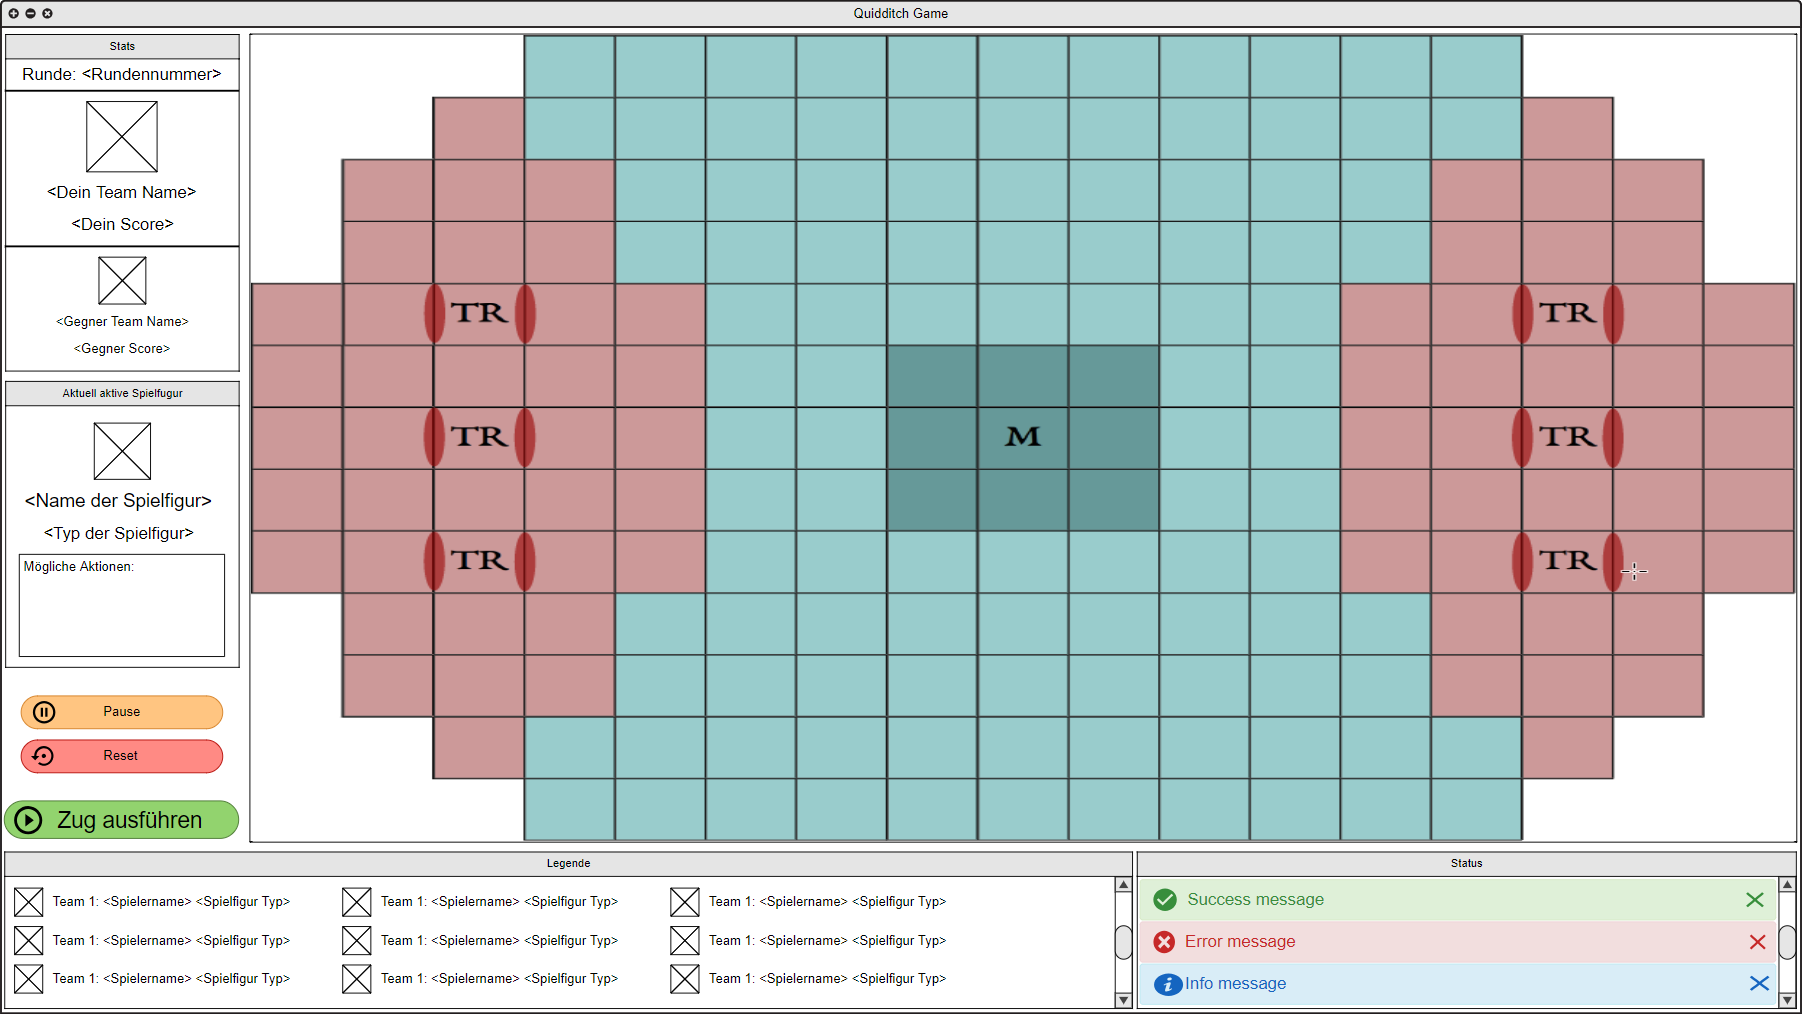
\includegraphics[width=\textwidth]{images/InGamePlayer.PNG}
    \end{figure}

    In der Spielansicht kann ein Spieler das aktuelle Spielgeschehen verfolgen und sein Züge ausführen. Dabei ist die Oberfläche in mehrere Teile unterteilt.\\
    Im \textit{Stats} Bereich werden grundlegende Informationen über die aktuelle Partie und die beiden Teams dargestellt. Das Team, das an oberster Position steht, ist momentan am Zug. Der darunter liegende Bereich ist der Bereich, in dem die \textit{aktuell ausgewählte Spielfigur} hervorgehoben wird. Dazu wird aufgeführt um welchen Typen von Spielfigur es sich handelt und welche grundlegenden Züge diese Figur ausführen kann. In den Fan Phasen werden hier vergleichbare Informationen zu den Fans angezeigt. Darunter befinden sich drei Buttons mit dem entweder das Spiel \textit{pausiert} werden , alle Veränderungen die man in der aktuellen Runde getätigt hat \textit{zurücksetzen} oder seinen Zug endgültig \textit{ausführen} kann. Am unteren Rand der Oberfläche ist eine \textit{Legende} mit einer Übersicht über alle Spielfiguren des eigenen und des gegnerischen Teams zu sehen. Daneben befindet sich ein Feld, in dem Statusmeldungen angezeigt werden können. Beispiele für solche Statusmeldungen sind eine Benachrichtigung über ein Faul oder über das erfolgreiche Ausführen eines Spielzuges. Der größte Teil der Oberfläche nimmt dass eigentliche Spielfeld ein. Hier werden alle Spielfiguren in den Feldern angezeigt auf denen sie sich gerade befinden. Ist man am Zug, so werden alle Züge, die von der aktuell ausgewählten Spielfigur ausgeführt werden können farblich hervor gehoben. Der Spieler kann diese Aktionen dann durch klicken ausführen. Ist man nicht am Zug so werden alle Eingabemöglichkeiten, mit Ausnahme des \textit{Pause} Buttons deaktiviert.
    

    \subsubsection{Spielansicht für einen Beobachter}
        
    \begin{figure}[H]
        \centering
        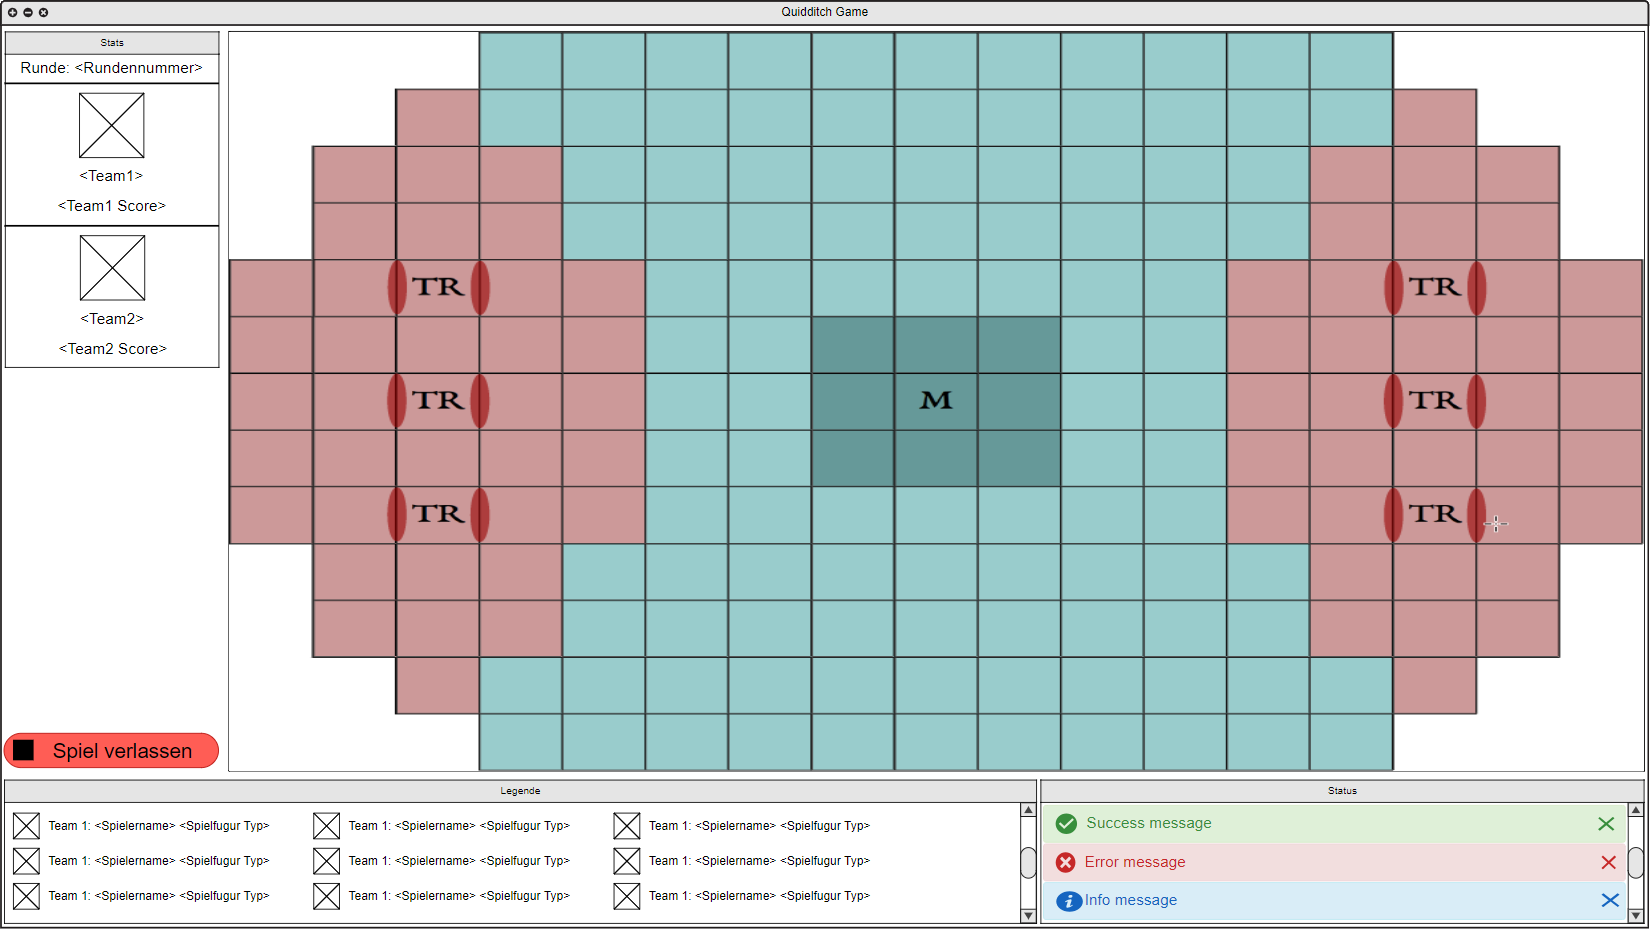
\includegraphics[width=\textwidth]{images/InGameObserver.PNG}
    \end{figure}

    In der Spielansicht kann ein Beobachter eine Partie wischen zwei anderen Gegnern passiv verfolgen. Die Oberfläche ist im wesentlichen gleich aufgebaut wie die Oberfläche, die die Spieler sehen. Jedoch sind beim Beobachter alle Felder die zur Eingabe dienen deaktiviert und teilweise ausgeblendet. Die einzige Interaktion, welche durch einen Button ermöglicht wird ist das vorzeitige \textit{verlassen} einer Partie.
    
    \subsubsection{Startbildschirm}
\begin{figure}[H]
	\centering
	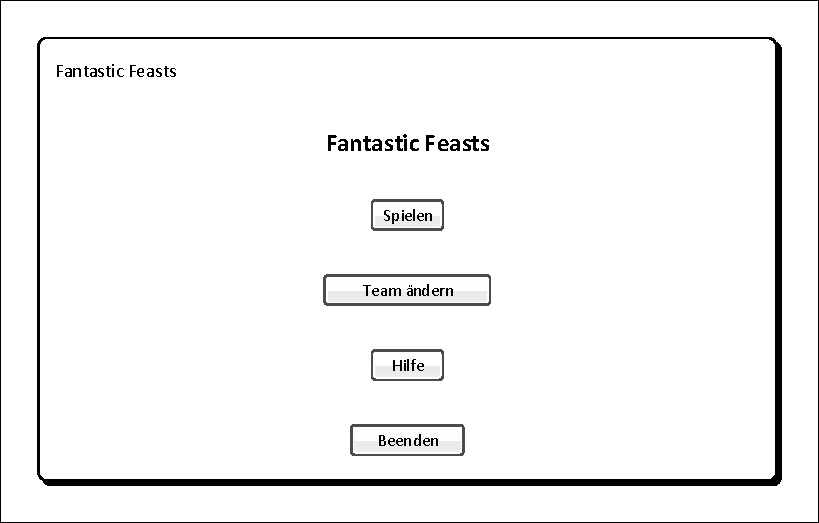
\includegraphics[scale=0.8]{images/Startbildschirm.pdf}
\end{figure}

Dieser Dialog erscheint nach Start der Anwendung. Der \glqq{}Spielen\grqq{}-Button öffnet den Spielsuche-Dialog. Der \glqq{}Team ändern\grqq{}-Button öffnet das \glqq{}Team ändern\grqq{}-Popup. Der \glqq{}Hilfe\grqq{}-Button öffnet den Hilfe-Dialog. Der \glqq{}Beenden\grqq{}-Button öffnet ein Bestätigungs-Popup und beendet bei positiver Antwort die Anwendung.

\subsubsection{Spielsuche}
\begin{figure}[H]
	\centering
	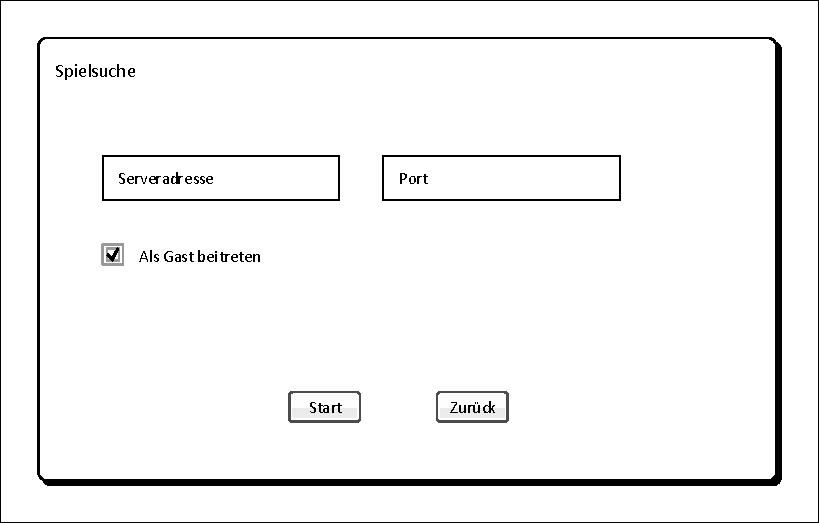
\includegraphics[scale=0.8]{images/Spielsuche.pdf}
\end{figure}

Der Benutzer gibt zuerst die Adresse und den Port des Spielservers und, mit dem er sich verbinden möchte. Wenn er die Partie beobachten will, wählt er \glqq{}Als Gast beitreten\grqq{} aus. Drückt er anschließend auf den \glqq{}Start\grqq{}-Button, versucht sich der Client mit dem angegebene Server zu verbinden. Mit dem \glqq{}Zurück\grqq{}-Button kann man zurück auf den Startbildschirm gelangen.
	
\subsubsection{Hilfe}
\begin{figure}[H]
	\centering
	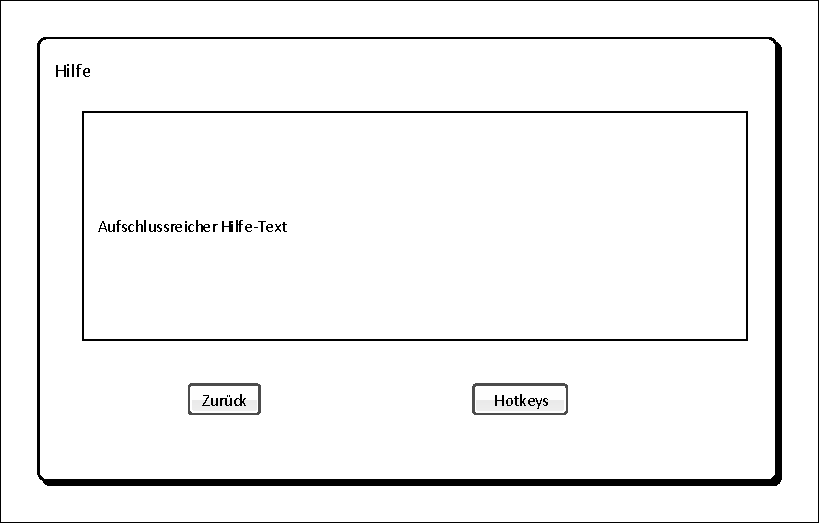
\includegraphics[scale=0.8]{images/Hilfe.pdf}
\end{figure}

In einem großen Textfeld, gegebenenfalls mit Scrollbar, wird ein Hilfetext angezeigt. Der \glqq{}Zurück\grqq{}-Button öffnet den Startbildschirm, der \glqq{}Hotkey\grqq{}-Button den Hotkey-Dialog.

\subsubsection{Hotkeys}
\begin{figure}[H]
	\centering
	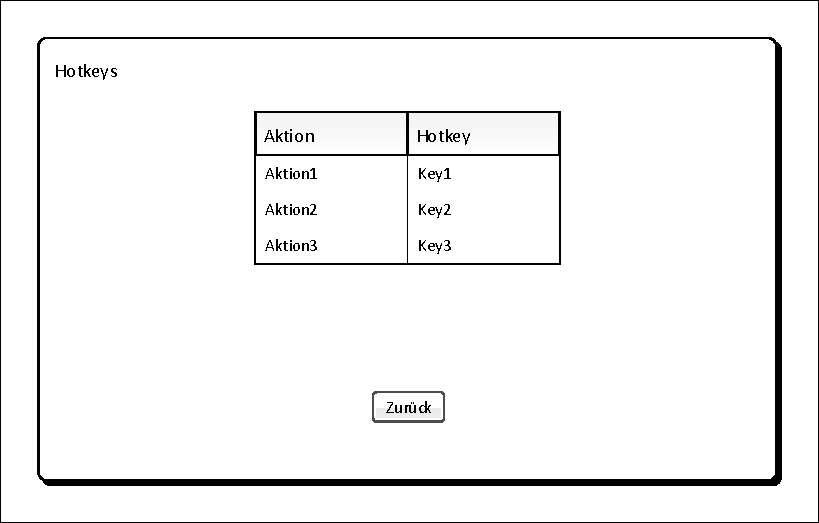
\includegraphics[scale=0.8]{images/Hotkeys.pdf}
\end{figure}

Hier werden alle verfügbaren Hotkeys in Tabellenform aufgelistet. Der \glqq{}Zurück\grqq{}-Button öffnet den Hilfe-Dialog.

\subsubsection{Team ändern}
\begin{figure}[H]
	\centering
	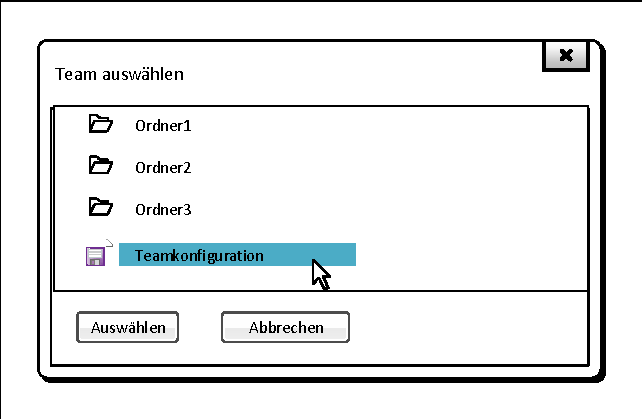
\includegraphics[scale=0.8]{images/Teamauswahl_Popup.pdf}
\end{figure}

In diesem Popup kann der Benutzer durch sein Dateisystem navigieren und eine JSON-Datei auswählen. Hat er eine gültige Datei ausgewählt und betätigt den \glqq{}Auswählen\grqq{}-Button, wird das Popup geschlossen und die Team-Konfiguration für das Spiel verwendet. Der \glqq{}Abbrechen\grqq{}-Button schließt das Popup und es werden keine Änderungen vorgenommen.

\subsubsection{Bestätigungsaufforderung}
\begin{figure}[H]
	\centering
	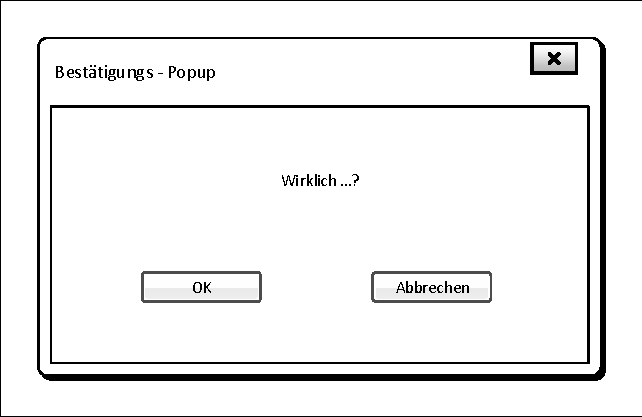
\includegraphics[scale=0.8]{images/OK_Popup.pdf}
\end{figure}

Dieser Aufbau wird für die Popups \glqq{}Beenden\grqq{} und \glqq{}Verlassen\grqq{} verwendet. Der \glqq{}Abbrechen\grqq{}-Button schließt das Popup und der Benutzer gelangt zurück in den Dialog, in dem er vor Öffnen des Popups war. Der "OK"-Button führt dazu, dass eine Aktion ausgeführt wird.

\subsubsection{Fehler}
\begin{figure}[H]
	\centering
	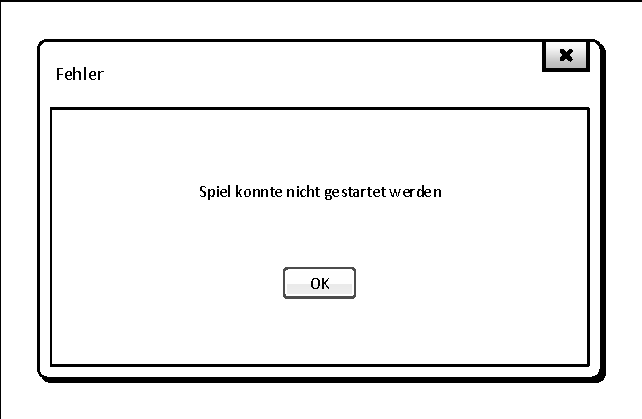
\includegraphics[scale=0.8]{images/Fehler_Popup.pdf}
\end{figure}

Dieser Aufbau wird für das Popup \glqq{}Spielstart fehlgeschlagen\grqq{} verwendet. Der angezeigt Text richtet sich nach dem aufgetretenen Fehler. Der \glqq{}OK\grqq{}-Button schließt das Popup.

\subsubsection{Pause}
\begin{figure}[H]
	\centering
	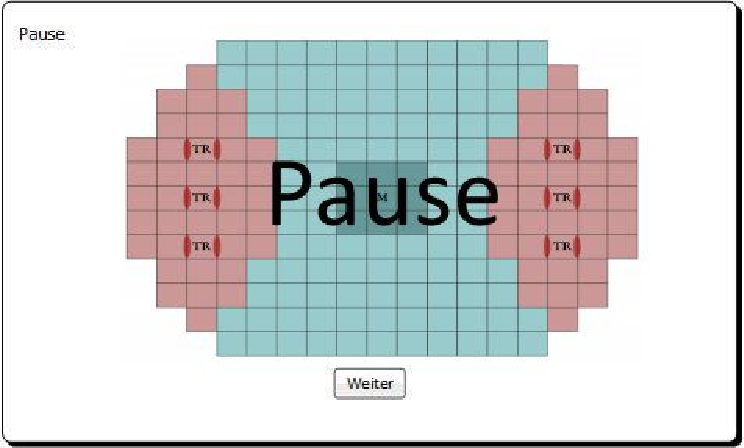
\includegraphics[scale=0.8]{images/Pause.pdf}
\end{figure}

Wird angezeigt, wenn das Spiel von einem Spieler pausiert wird. Der \glqq{}Weiter\grqq{}-Button setzt die Partie fort und kann nicht von einem Gast betätigt werden.

\subsubsection{Verbindungsabbruch}
\begin{figure}[H]
	\centering
	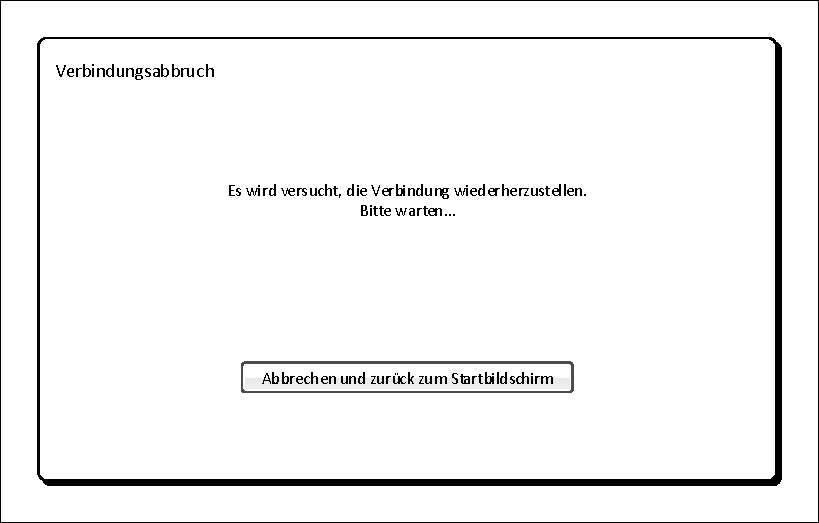
\includegraphics[scale=0.8]{images/Verbindungsabbruch.pdf}
\end{figure}

Im Falle eines Verbindungsabbruchs zwischen Client und Server wird dieser Dialog angezeigt. Wird die Verbindung wiederhergestellt, gelangt der Benutzer automatisch wieder zurück in den vorherigen Dialog. Alternativ kann er durch betätigen des Buttons zum Startbildschirm gelangen. Ist er ein Spieler, kann er die Partie nicht weiterführen und sein Gegner gewinnt nach Ablauf einer Zeitdauer die Partie.

\subsubsection{Spielende}
\begin{figure}[H]
	\centering
	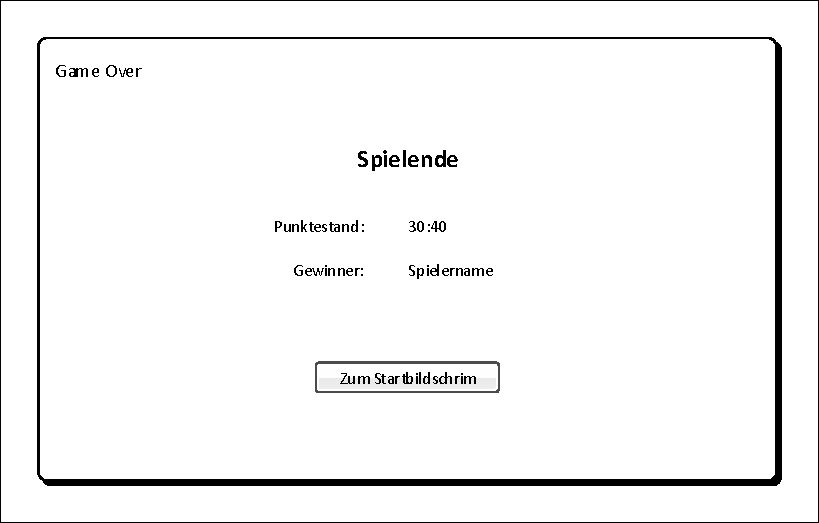
\includegraphics[scale=0.8]{images/Spielende.pdf}
\end{figure}

Bei Spielende wird dieser Dialog geöffnet. Hier werden der Punktestand bei Spielende und der Name des Gewinners angezeigt. Der Button öffnet den Startbildschirm-Dialog.
